\subsection{Introducción}

Sharding es la solución que utiliza MongoDB para brindar un acceso a la información almacenada en un tiempo razonable
a medida que aumenta el volumen de datos. 
Permite escalar horizontalmente, es decir agregar nuevas computadoras para distribuir la información.
A continuación describimos a grandes rasgos el funcionamiento de este sistema, se evita entrar en ciertos detalles
específicos de los algoritmos y procesos involucrados porque no resulta fundamental para entender la solución propuesta.\\

\subsection{Estructura de un sharded cluster}

Una colección es dividida en subconjuntos denominados "shards" (se debe configurar un campo del esquema como `shard key'), cada shard
contiene chunks que poseen información en un rango del shard key configurado, de esta manera la información con una shard key similar
se mantendrá próxima (en la mayoría de los casos). 

\begin{figure}[h!]
 \centering
 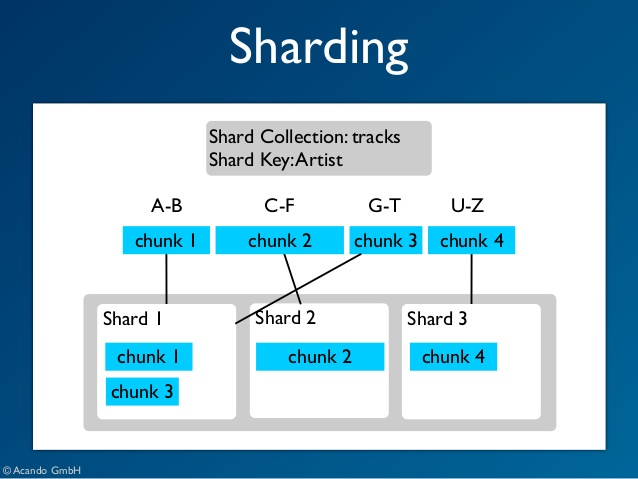
\includegraphics[scale=0.35,keepaspectratio=true]{./sharding.jpg}
 % sharding.jpg: 638x479 pixel, 72dpi, 22.51x16.90 cm, bb=0 0 638 479
 \caption{Diagrama de sharding}
\end{figure}


Por ejemplo, si en una colección se elige `mes del año' como `shard key', y tengo tres
chunks, para el primer rango puedo tener los datos de Enero a Abril, para el segundo de Abril a Agosto, y el último de Agosto a Diciembre.
A medida que se agregue información, puede suceder que se dividan estos chunks, y quede por ejemplo un chunk por mes del año.
A partir de ese momento no será posible dividir para formar nuevos rangos, por lo tanto los chunks se vuelven cada vez más grandes.

\begin{figure}[h!]
 \centering
 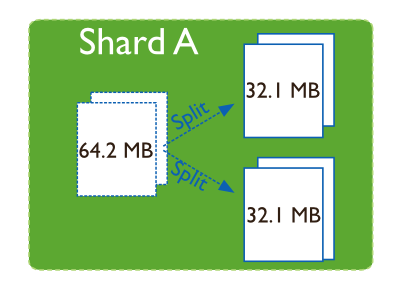
\includegraphics[scale=0.5,keepaspectratio=true]{./split-chunk.png}
 % split-chunk.png: 400x288 pixel, 72dpi, 14.11x10.16 cm, bb=0 0 400 288
 \caption{Division de chunk}
\end{figure}

\subsection{Balanceo y migración}

Los shards se distribuirán en diferentes servidores, lo deseable es contar con la información distribuida de la mejor forma
posible para optimizar las lecturas y escrituras. Además de dividirse, un chunk puede ser migrado de un shard a otro, de 
esta forma se busca balancear la carga entre los servidores.


\begin{figure}[h!]
 \centering
 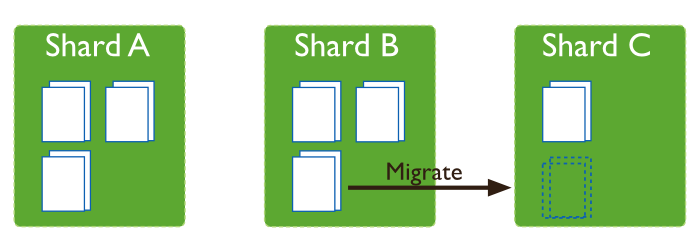
\includegraphics[scale=1,keepaspectratio=true]{./sharding-migrating.png}
 % sharding-migrating.png: 700x252 pixel, 126dpi, 14.11x5.08 cm, bb=0 0 400 144
 \caption{Migración de chunk}
\end{figure}


\subsection{Elección de `Shard key'}

A partir de lo desarrollado, podemos concluir que si queremos utilizar sharding en nuestra colección, resulta fundamental
escoger una `shard key' apropiada.
No hay manera de elegir una clave perfecta, para eso se tienen en cuenta una serie de criterios sobre como se comportan los
datos que manejamos.\\

\begin{itemize}
\item 
Cardinalidad: que tanto puede dividirse el rango de valores, lo deseable es tener una cardinalidad alta, es decir que pueda
generar gran cantidad de rangos. Un ejemplo de alta cardinalidad sería el DNI, de baja puede ser el código de provincia (en
última instancia siempre hay que tener en cuenta el contexto en el que se usan los datos).
\item 
Distribución de las escrituras: lo ideal es distribuir las escrituras de manera uniforme entre los shards, si se escoge una
clave que crece de manera monótona, resulta en un exceso de inserts sobre un único shard.
\item 
Distribución de las lecturas: como en el caso de las escrituras, queremos obtener distribución uniforme.
\item 
Tipo de consultas: tener en cuenta que consultas se realizarán sobre la colección, si involucra búsqueda por rango o un documento
en particular, en cualquier caso lo deseable es que se accedan la menor cantidad de shards posibles. Para eso es necesario
que la shard key esté presente en la consulta efectuada. Por ejemplo si quiero consultar documentos por mes, puedo configurar
una 'shard key' compuesta por mes y algún otro campo, de esta forma la información de un mes en particular estará almacenada en un mismo shard
(de vuelta depende del caso, pero en general sucedería así).\end{itemize}


\subsection{Implementación}

Se utiliza la arquitectura de prueba
\begin{figure}[h!]
 \centering
 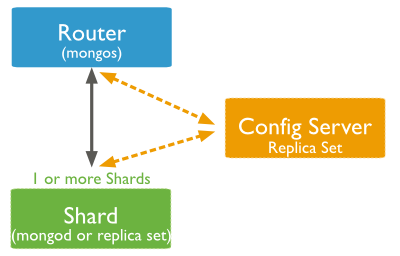
\includegraphics[scale=0.5,keepaspectratio=true]{./sharded-cluster-test-architecture.png}
 % sharded-cluster-test-architecture.png: 400x256 pixel, 72dpi, 14.11x9.03 cm, bb=0 0 400 256
 \caption{Test Architecture}
\end{figure}

Trabajando sobre publicaciones con el siguiente esquema.
{AGREGAR ESQUEMA}

Generamos los datos de forma aleatoria(uniformemente) sobre un período de años acotado (5 años), `tipo de publicación' puede tomar tres valores
(servicios, artículos y mixta).
Creamos tres shards para la colección:

\begin{enumerate}
\item 
En primera instancia escogimos `tipo de publicación' como shard key. Obtuvimos una distribución pareja, ya que eran 3 shards
para 3 rangos posibles. A simple vista podría parecer una buena clave, pero hay que tener en cuenta que los datos reales
podrían tener otra distribución, y la baja cardinalidad en ese caso sería un problema, suponiendo un 90\% de publicaciones de artículos 
implicaría tener los shards totalmente desbalanceados.
{Gráficos de tipo de publicación}
\item 
Luego escogimos otro índice simple, en este caso la fecha, que resultó más interesante que el anterior. A medida que se insertaron los 
datos se puede observar como se produce el balanceo de shards a través de la división y migración de los chunks, ya que es una clave con 
cardinalidad alta. Hay que tener en cuenta que los datos fueron generados de forma aleatoria, quizás en un caso real las fechas serían 
consecutivas lo que deriva en que las inserciones apunten al mismo shard.
{Gráficos de fechas}
\item 
Por último se utiliza un índice hash sobre el campo `id' que genera Mongo a cada documento.\end{enumerate}


\subsection{Conclusión}
\subsection{Fuentes} 
\begin{enumerate}
\item 
https://docs.mongodb.com/v3.0/sharding/
\item 
https://www.mongodb.com/blog/post/on-selecting-a-shard-key-for-mongodb
\item 
http://www.mongodbspain.com/es/tag/shard/\end{enumerate}



